\documentclass{article}
\usepackage[nottoc,numbib]{tocbibind}
\usepackage[utf8]{inputenc}
\usepackage{graphicx} 
\usepackage[a4paper, left=2cm, right=2cm, top=3cm, bottom=3cm]{geometry}
\usepackage[table]{xcolor}
\usepackage{algorithm}
\usepackage{algpseudocode}
\usepackage{placeins}
\usepackage{float}
\usepackage{listings}
\usepackage{xcolor}
\usepackage{polski}
\usepackage{graphicx}
\usepackage{subcaption}

\definecolor{light-gray}{gray}{0.95} % Define the shade of gray you want

\lstset{
    language=bash,
    backgroundcolor=\color{light-gray}, % Set the background color
    basicstyle=\ttfamily,
    breaklines=true
}

\title{MBI - Analiza danych sekwencyjnych człowieka}
\author{Mateusz Krakowski, Bartosz Latosek}
\date{23 Maja 2024}

\begin{document}

\maketitle

\section{Liczenie pokrycia}
Przygotowano pliki zgodnie z instrukcją.

Pierwsze 10 wierszy bedFile:
\begin{lstlisting}[language=R]
> (fread(bedFile)
fread(bedFile) 
     V1       V2       V3
  1: 22 21345867 21346168
  2: 22 21346453 21346708
  3: 22 21347033 21347243
  4: 22 21347901 21348093
  5: 22 21348163 21348608
  6: 22 21348797 21349066
  7: 22 21349109 21349365
  8: 22 21349985 21350451
  9: 22 21350935 21351305
 10: 22 21351471 21351687
...
\end{lstlisting}
Podsumowanie:
\begin{lstlisting}[language=R]
> summary(apply(Y_ac, 2, median))
   Min. 1st Qu.  Median    Mean 3rd Qu.    Max.
  21.06   24.04   25.29   27.37   27.08   76.03
\end{lstlisting}



\subsection{Która próbka ma najmniejsze, a która największą medianę głębokości pokrycia?}
Do obliczenia tego wykorzystano funkcje:
\begin{lstlisting}[language=R]
sample_medians <- apply(Y_ac, 2, median)

smallest_median_index <- which.min(sample_medians)

largest_median_index <- which.max(sample_medians)
\end{lstlisting}

Najmniejsza Mediana dla NA18991:
\begin{lstlisting}[language=R]
> smallest_median_index
NA18991
     25
\end{lstlisting}
Największa Mediana dla NA19137:
\begin{lstlisting}[language=R]
> largest_median_index
NA19137
     29
\end{lstlisting}

\section{Wykrywanie zmian liczby kopii DNA przy użyciu na-
rzędzia CODEX}
Załadowano dane:
\begin{lstlisting}[language=R]
> colnames(cdf) <- c("Chr", "Start", "S
f$SampleNa> cdf <- cdf[order(cdf$Sample
> dim(cdf)
[1] 465498      5
> head(cdf)
   Chr  Start   Stop ReadCount SampleNa
1:  20  68319  68439       103    NA069
2:  20  76611  77091       129    NA069
3:  20 123208 123358        69    NA069
4:  20 125995 126389       105    NA069
5:  20 138119 138269        37    NA069
6:  20 139359 139719       156    NA069
> bedFile <- paste0(workDir, "data/bed/
> sampname <- unique(cdf$SampleName)
\end{lstlisting}

\subsection{Ile eksonów (regionów) zostało usuniętych w wyniku kontroli jakości?}
Przeprowadzono kontrolę jakości:
\begin{lstlisting}[language=R]
> qcObj <- qc(Y, sampname, chr, ref, mapp, gc,
+ cov_thresh = c(cov_thresh_from, cov_thresh_to),
+ length_thresh = c(length_thresh_from, length_thresh_to),
+ mapp_thresh = mapp_thresh,
+ gc_thresh = c(gc_thresh_from, gc_thresh_to))
Excluded 279 exons due to extreme coverage.
Excluded 18 exons due to extreme exonic length.
Excluded 22 exons due to extreme mappability.
Excluded 15 exons due to extreme GC content.
After taking union, excluded 318 out of 4702 exons in QC.
\end{lstlisting}
W wyniku kontroli jakości usuniętych zostało 318 z 4702 eksonów.
\subsection{Ile eksonów (regionów) będzie usuniętych jeżeli zmienimy progi odcięcia zawartości GC (gc\_thresh\_from, gc\_thresh\_to)? Podaj wynik dla wybranych przez Ciebie progów.}
\begin{lstlisting}[language=R]
> gc_thresh_from <- 30
> gc_thresh_to <- 70 
> qcObj <- qc(Y, sampname, chr, ref, mapp, gc,
+ cov_thresh = c(cov_thresh_from, cov_thresh_to),
+ length_thresh = c(length_thresh_from, length_thresh_to),       
+ mapp_thresh = mapp_thresh,
+ gc_thresh = c(gc_thresh_from, gc_thresh_to))
Excluded 279 exons due to extreme coverage.
Excluded 18 exons due to extreme exonic length.
Excluded 22 exons due to extreme mappability.
Excluded 324 exons due to extreme GC content.
After taking union, excluded 472 out of 4702 exons in QC. 
\end{lstlisting}
W wyniku zmiany progów na wartość gc\_thresh\_from = 30 i gc\_thresh\_to = 70 ilość usuniętych eksonów zwiększyła się do 472 egzemplarzy.
\begin{lstlisting}[language=R]
> gc_thresh_from <- 40
> gc_thresh_to <- 60 
> qcObj <- qc(Y, sampname, chr, ref, mapp, gc,
+ cov_thresh = c(cov_thresh_from, cov_thresh_to),
+ length_thresh = c(length_thresh_from, length_thresh_to),       
+ mapp_thresh = mapp_thresh,
+ gc_thresh = c(gc_thresh_from, gc_thresh_to))
Excluded 279 exons due to extreme coverage.
Excluded 18 exons due to extreme exonic length.
Excluded 22 exons due to extreme mappability.
Excluded 2088 exons due to extreme GC content.
After taking union, excluded 2170 out of 4702 exons in QC.  
\end{lstlisting}
Dalsze zwiększanie gc\_thresh\_from i zmniejszanie gc\_thresh\_to powoduje zwiększenie się liczby usuniętych eksonów.
\begin{lstlisting}[language=R]
> gc_thresh_from <- 10
> gc_thresh_to <- 90
> qcObj <- qc(Y, sampname, chr, ref, mapp, gc,
+ cov_thresh = c(cov_thresh_from, cov_thresh_to),
+ length_thresh = c(length_thresh_from, length_thresh_to),
+ mapp_thresh = mapp_thresh,
+ gc_thresh = c(gc_thresh_from, gc_thresh_to))
<- qcObj$Y_qc; sampname_qc <- qcObj$sampname_qc; gc_qc <- qcObj$gc_qc
mapp_qc <- qcObj$mapp_qc; ref_qc <- qcObj$ref_qc; qcmat <- qcObj$qcmat
Excluded 279 exons due to extreme coverage.
Excluded 18 exons due to extreme exonic length.
Excluded 22 exons due to extreme mappability.
Excluded 2 exons due to extreme GC content.
After taking union, excluded 318 out of 4702 exons in QC. 
\end{lstlisting}

Zmniejszenie gc\_thresh\_from i zwiększenie gc\_thresh\_to  nie spowodowało zmniejszenia się liczby odrzucanych eksonów z uwagi na to, że zmniejszyła się jedynie liczba odrzuconych z uwagi na ekstremalną wartość GC, część wspólna zbioru nieodrzuconych pozostała taka sama.

Przeprowadzono normalizację głębokości pokrycia oraz segmentację dla wartości: \\ gc\_thresh\_from = 20 i gc\_thresh\_to = 80.
\begin{lstlisting}[language=R]
> head(finalcall)
  sample_name chr cnv    st_bp    ed_bp length_kb st_exon ed_exon raw_cov
1     NA07000  20 dup 60908921 60909439     0.519    3945    3946     417
2     NA07000  20 dup 60921546 60926868     5.323    3954    3957     474
3     NA07357  20 del  1638233  1896162    257.93     126     127      90
4     NA10851  20 del 22562688 22564923     2.236    1208    1209     515
5     NA10851  20 dup 60881686 60883534     1.849    3899    3903     721
6     NA10851  20 dup 62571460 62574104     2.645    4289    4292     501
  norm_cov copy_no  lratio    mBIC targetCount
1      286       3  26.072   6.312           1
2      346       3  19.183   7.148           3
3      226       1  50.621   31.45           1
4      931       1 108.555  88.397           1
5      513       3  35.828 103.755           4
6      344       3   31.13 115.414           3
> nrow(finalcall)
[1] 438
> nrow(finalcall[finalcall$cnv=='del',])
[1] 174
> nrow(finalcall[finalcall$cnv=='dup',])
[1] 264
> nrow(finalcall[finalcall$cnv=='del' & finalcall$copy_no==0,])
[1] 3
\end{lstlisting}

\subsection{Ile zmian liczby kopii wykrył CODEX?}
\begin{lstlisting}[language=R]
> nrow(finalcall)
[1] 438
\end{lstlisting}
CODEX wykrył 438 zmian liczby kopii.
\subsection{Ile wśród nich jest delecji a ile duplikacji?}
\begin{lstlisting}[language=R]
> nrow(finalcall[finalcall$cnv=='del',])
[1] 174
> nrow(finalcall[finalcall$cnv=='dup',])
[1] 264
\end{lstlisting}
Delecji jest 174, duplikatów jest 264.
\subsection{Czy występują jakiekolwiek homozygotyczne delecje (copy\_no ==0)?}
\begin{lstlisting}[language=R]
> nrow(finalcall[finalcall$cnv=='del' & finalcall$copy_no==0,])
[1] 3
\end{lstlisting}
Istnieją 3 delecje homozygotyczne.


\subsection{Wykresy dla numerów zmiany(numer zmiany pod wykresem)}

\begin{figure}[H]
    \centering
    \begin{subfigure}{0.48\textwidth}
        \centering
        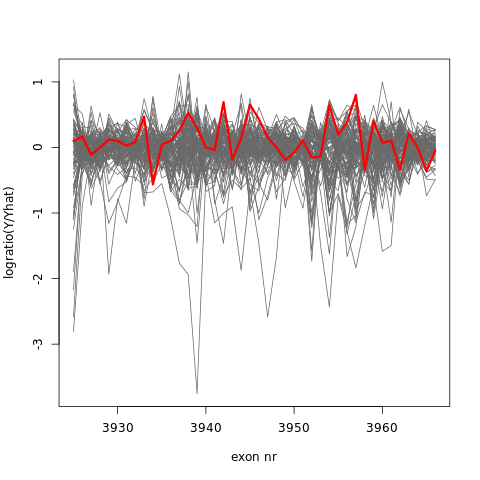
\includegraphics[width=\linewidth]{img/cnv1.png}
        \caption{cnvId = 1}
        \label{fig:sub1}
    \end{subfigure}
    \hfill
    \begin{subfigure}{0.48\textwidth}
        \centering
        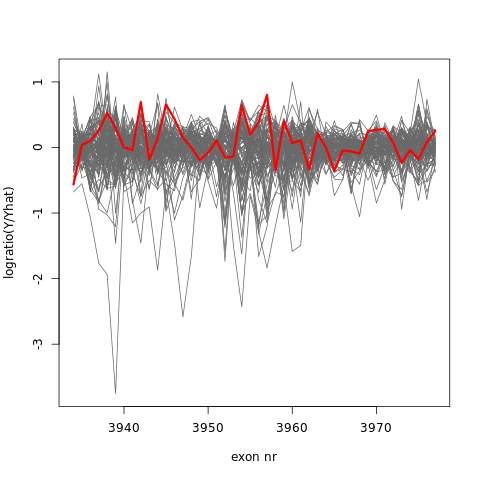
\includegraphics[width=\linewidth]{img/cnv2.png}
        \caption{cnvId = 2}
        \label{fig:sub2}
    \end{subfigure}
    
    \begin{subfigure}{0.48\textwidth}
        \centering
        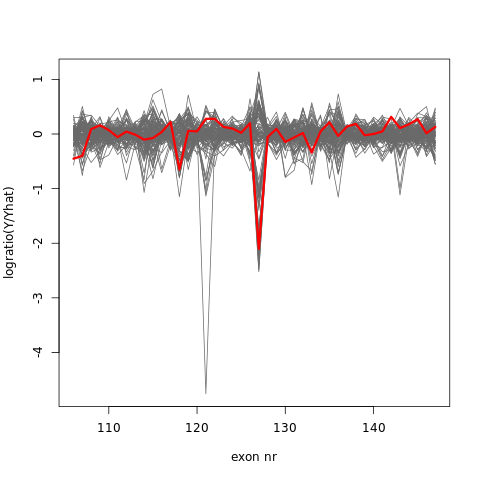
\includegraphics[width=\linewidth]{img/cnv3.png}
        \caption{cnvId = 3}
        \label{fig:sub3}
    \end{subfigure}
    \hfill
    \begin{subfigure}{0.48\textwidth}
        \centering
        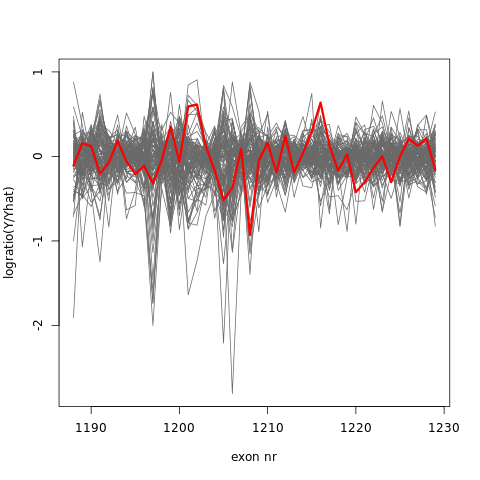
\includegraphics[width=\linewidth]{img/cnv4.png}
        \caption{cnvId = 4}
        \label{fig:sub4}
    \end{subfigure}
    
    \label{fig:combined}
\end{figure}
\section{Zadanie implementacyjne}
\begin{lstlisting}[language=Python]
import argparse
import pandas as pd

def main(path_finalcall, path_dgv):
    dgv_data = pd.read_csv(path_dgv, header=0, sep='\t',
                         dtype={'chr': str, 'start': int, 'end': int, 'variantsubtype': str, 'samples': str})
    dgv_data = dgv_data[['chr', 'start', 'end', 'variantsubtype', 'samples']]
    dgv_data = dgv_data[dgv_data['chr'] == '20']

    cnv_data = pd.read_csv(path_finalcall, sep=',')
    cnv_data = cnv_data[['sample_name', 'chr', 'st_bp', 'ed_bp', 'cnv']]

    deletion_overlapping_count, duplication_overlapping_count, overlapping_more_than_80_count = 0, 0, 0

    for _, cnv_row in cnv_data.iterrows():
        print(cnv_row['sample_name']) # show sample name
        x1, x2 = cnv_row['st_bp'], cnv_row['ed_bp']
        for _, dgv_row in dgv_data.iterrows():
            y1, y2 = dgv_row['start'], dgv_row['end']
            if max(x1, y1) <= min(x2, y2):
                if dgv_row['variantsubtype'] == 'deletion':
                    deletion_overlapping_count += 1
                if dgv_row['variantsubtype'] == 'duplication':
                    duplication_overlapping_count += 1
                if min(x2, y2) - max(x1, y1) >= 0.8 * (y2 - y1):
                    overlapping_more_than_80_count += 1


    print(f'Overlapping deletions: {deletion_overlapping_count}')
    print(f'Overlapping duplications: {duplication_overlapping_count}')
    print(f'Any changes overlapping by more than 80%: {overlapping_more_than_80_count}')

if __name__ == '__main__':
    parser = argparse.ArgumentParser(description='Process some files.')
    parser.add_argument('finalcall', type=str, help='Path to finalcall file')
    parser.add_argument('dgv', type=str, help='Path to dgv file')

    args = parser.parse_args()

    main(args.finalcall, args.dgv)

\end{lstlisting}

Program korzysta z biblioteki argparse, aby go uruchomić należy podać ścieżki do pliku wejściowych w następujący sposób:
\begin{lstlisting}[language=bash]
python .\program.py finalcall.csv GRCh37_hg19_variants_2020-02-25.txt
\end{lstlisting}

Wyjście programu:
\begin{lstlisting}[language=bash]
... # sample names so we can see that the script is working, ex. NA19099
Overlapping deletions: 2684
Overlapping duplications: 562
Any changes overlapping by more than 80%: 5729
\end{lstlisting}
\subsection{Ile delecji z DGV ma jakąkolwiek część wspólną z zadanym CNV?}
2684 delecji ma część wspólną z zadanym CNV.
\subsection{Ile duplikacji z DGV ma jakąkolwiek część wspólną z zadanym CNV?}
562 duplikacji ma część wspólną z zadanym CNV.
\subsection{Ile dowolnych zmian z DGV ma 80-procentową część wspólną z zadanym CNV?}
5729 dowolnych zmian z DGV ma 80-procentową część wspólną z zadanym CNV.




\end{document}
